\documentclass[12pt, a4paper]{article}

\usepackage[czech]{babel}
\usepackage{lmodern}
\usepackage[utf8]{inputenc}
\usepackage[T1]{fontenc}
\usepackage[pdftex]{graphicx}
\usepackage{amsmath}
\usepackage[hidelinks,unicode]{hyperref}
\usepackage{float}
\usepackage{listings}
\usepackage{tikz}
\usepackage{xcolor}
\usepackage[final]{pdfpages}


\definecolor{mauve}{rgb}{0.58,0,0.82}
\usetikzlibrary{shapes,positioning,matrix,arrows}

\newcommand{\img}[1]{(viz obr. \ref{#1})}

\definecolor{pblue}{rgb}{0.13,0.13,1}
\definecolor{pgreen}{rgb}{0,0.5,0}
\definecolor{pred}{rgb}{0.9,0,0}
\definecolor{pgrey}{rgb}{0.46,0.45,0.48}

\lstset{frame=tb,
  language=C,
  aboveskip=3mm,
  belowskip=3mm,
  showstringspaces=false,
  columns=flexible,
  basicstyle={\small\ttfamily},
  numbers=none,
  numberstyle=\tiny\color{gray},
  keywordstyle=\color{blue},
  commentstyle=\color{dkgreen},
  stringstyle=\color{mauve},
  breaklines=true,
  breakatwhitespace=true,
  tabsize=3
}


\let\oldsection\section
\renewcommand\section{\clearpage\oldsection}

\begin{document}
	% this has to be placed here, after document has been created
	% \counterwithout{lstlisting}{chapter}
	\renewcommand{\lstlistingname}{Ukázka kódu}
	\renewcommand{\lstlistlistingname}{Seznam ukázek kódu}
    \begin{titlepage}

        \centering

        \vspace*{\baselineskip}
        \begin{figure}[H]
        \centering
        
\includegraphics[width=7cm]{img/fav-logo.jpg}
        \end{figure}

        \vspace*{1\baselineskip}

        \vspace{0.75\baselineskip}

        \vspace{0.5\baselineskip}
        {Semestrální práce z předmětu KIV/OS}

        {\LARGE\sc Simulace operačního systému\\}

        \vspace{4\baselineskip}

        \vspace{0.5\baselineskip}

        {\sc\Large Eliška Mourycová \\}
        \vspace{0.5\baselineskip}
        {A20N0061P}

        {\sc\Large Ondřej Drtina \\}
        \vspace{0.5\baselineskip}
        {A20N0077P}

        {\sc\Large Stanislav Král \\}
        \vspace{0.5\baselineskip}
        {A20N0091P}

        \vfill

        {\sc Západočeská univerzita v Plzni\\
        Fakulta aplikovaných věd}

    \end{titlepage}


    % TOC
    \tableofcontents
    \pagebreak

    
    \section{Analýza}
    % TODO analýza

    \section{Kernel}

    Kernel je část operačního systému, která provádí inicializaci hardwaru, zajišťuje správu prostředků a umožňuje vytvářet programy či vlákna. Uživatelskému prostoru nabízí své služby pomocí tzv. systémových volání. V této semestrální práci lze kernel rozdělit do následujících částí: 
\begin{itemize}
    \item správa procesů/vláken
    \item správa otevřených souborů
    \item souborový systém FAT12
\end{itemize}

\subsection{Správa procesů a vláken}
Tuto část kernelu lze považovat za nejdůležitější, jelikož bez její přítomnosti by nebylo možné spouštět žádné programy. Stará se o vytváření procesů a jejich správu, kdy lze procesy synchronizovat a nastavovat jejich návratové hodnoty. Simulace vláken a procesů je realizována pomocí konstrukcí pro vytváření vláken ze standardní knihovny \texttt{thread}. Většina kódu této části se nachází v souboru \texttt{/kernel/process.cpp}.

Pro použití služeb této části kernelu z uživatelského prostoru slouží následující systémová volání ze skupiny \texttt{Process}.

\begin{itemize}
    \item \texttt{Clone},
    \item \texttt{Wait\_For},
    \item \texttt{Read\_Exit\_Code},
    \item \texttt{Exit},
    \item \texttt{Register\_Signal\_Handler}
\end{itemize}

\subsubsection{Vytvoření nového vlákna}

Nativní identifikátory vytvořených vláken jsou mapovány na typ \texttt{kiv\_os::THandle}, který se dále používá v rámci kernelu jako interní identifikátor vláken.

Při zpracování požadavku na vytvoření nového vlákna se ze vstupních registrů načtou potřebné argumenty, a zavolá se funkce \texttt{run\_in\_a\_thread}, která přebírá argument obsahující vstupní bod části kódu, jež se má spustit v novém vlákně. Tato funkce vytvoří nové \texttt{std::thread} vlákno, kterému jako vstupní funkci nastaví funkci \texttt{thread\_entrypoint} přebírající skrz argumenty vstupní bod kódu ke spuštění. Uvnitř spuštěného vlákna se před vykonáváním kódu dále čeká dokud kernel nepřidá toto vlákno do tabulky všech vláken. Čekání je realizováno pomocí semaforu, a teprve po jeho notifikaci se začne vykonávat požadovaný kód. 

Při vytváření nového vlákna se navíc ještě dohledává jaké vlákno či proces nové vlákno vytváří. Tato informace se později např. využívá při změně pracovního adresáře procesu.

\subsubsection{Synchronizace vláken}
Jádro umožňuje synchronizaci vytvořených vláken pomocí systémového volání \texttt{Wait\_For}. Obsluha tohoto volání je realizována pomocí funkce \texttt{wait\_for}, která přebírá pole obsahující identifikátory vláken, na která se má čekat. Synchronizace je realizována pomocí semaforů, kdy ke každému běžícímu vláknu je veden seznam semaforů, které se mají při skončení vlákna notifikovat. Jeden semafor může tedy být přiřazen k více než jednomu vláknu. 

Na začátku obsluhy je k daným vláknům přiřazen nově vytvořený semafor, a zahájí se čekání na notifikaci tohoto semaforu. V moment, kdy je daný semafor notifikován, je vlákno čekající na semafor probuzeno, a tento semafor je odebrán ze všech ostatních seznamů, kde se vyskytuje. Spolu s notifikací semaforu je čekajícímu vláknu předána i informace o tom, jaké vlákno semafor probudilo. 

\begin{figure}[!ht]
\centering
{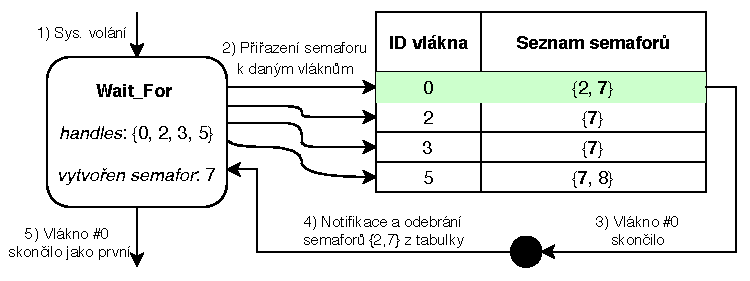
\includegraphics[width=14.5cm]{pdf/wait_for.pdf}}
\caption{Zjednodušený diagram obsluhy sys. volání \texttt{Wait\_For}}
\label{fig:screen-transition-diagram}
\end{figure}

\subsubsection{Vytváření procesů}
Vytváření procesů je principiálně stejné jako vytváření vláken, a používá se stejných funkcí jako při vytváření nového vlákna. Hlavním rozdílem je to, že až v jádře se převádí název programu na vstupní bod programu, který se předává funkci \texttt{run\_in\_a\_thread}. Před zahájením vykonávání kódu programu je po vytvoření nového vlákna dle jeho identifikátoru přidán nový záznam do tabulky všech procesů. Dále také nový proces dědí pracovní adresář od procesu, kterým byl vytvořen.

Tabulka procesů, která je v kódu implementována třídou \texttt{Process\_Control\_Block}, obsahuje následující sloupce:
\begin{itemize}
    \item \texttt{kiv\_os::THandle handle} - identifikátor (\textbf{PID}\footnote{process identifier}) procesu,
    \item \texttt{kiv\_os::THandle std\_in} - identifikátor standardního vstupu procesu,
    \item \texttt{kiv\_os::THandle std\_out} - identifikátor standardního výstupu procesu,
    \item \texttt{char *program\_name} - název programu, který proces vykonává,
    \item \texttt{std::filesystem::path working\_directory} - aktuální pracovní adresář procesu,
    \item \texttt{kiv\_os::NOS\_Error exit\_code} - návratová hodnota procesu programu, který proces vykonává,
    \item \texttt{Process\_Status status} - stav procesu, který může nabývat hodnot \texttt{Ready}, \texttt{Running}, \texttt{Zombie}
\end{itemize}

Předtím, než proces začne vykonávat kód programu, tak setrvává ve stavu \texttt{Process\_Status::Ready}. Během vykonávání programu setrvává ve stavu \texttt{Process\_Status::Running}. Pokud proces již dokončil vykonávání kódu programu, tak setrvává ve stavu \texttt{Process\_Status::Zombie}, dokud si jiný proces nepřečte jeho návratovou hodnotu. 

\subsubsection{Nastavení návratové hodnoty procesu}
Všem procesům je při jejich vytvoření nastaven výchozí návratovou hodnotu \texttt{kiv\_os\\::NOS\_Error::Success}. V případě, že nějaký program chce tuto hodnotu nastavit ručně, tak má možnost použít systémové volání \texttt{Exit}, a v registrech nastavit požadovanou návratovou hodnotu.

\subsubsection{Přečtení návratové hodnoty procesu}
Přečtení návratové hodnoty procesu z uživatelského prostoru je možné pomocí systémového volání \texttt{Read\_Exit\_Code}, kdy je před voláním nutné nastavit do registrů identifikátoru procesu, jehož návratovou hodnotu chceme přečíst.

Toto volání je implementováno tak, že se nejdřív zkontroluje, zdali daný proces již skončil a setrvává ve stavu \texttt{Process\_Status::Zombie}. Pokud ano, tak se jednoduše získá z tabulky jeho návratová hodnota. V případě, že proces ještě neskončil, tak v tomto stavu nesetrvává, a tudíž nelze v tuto chvíli přečíst jeho návratovou hodnotu, protože by se ještě mohla změnit. Obsluha systémového volání \texttt{Read\_Exit\_Code} tedy zavolá funkci \texttt{wait\_for} a počká, dokud daný proces neskončí. Poté přečte a vrátí jeho návratovou hodnotu.

 Na konci tohoto volání po úspěšném přečtení návrtové hodnoty je z tabulky procesů daný proces, jehož návratovou hodnotu jsme přečetli, odebrán.

\subsubsection{Nastavení obsluhy systémového signálu aktuálního procesu}
Aby každý proces mohl nastavit vlastní obsluhu libovolného systémového signálu, tak jádro poskytuje možnost volat systémové volání \texttt{Register\_Signal\_Handler}.

Kontrakt definovaný v \texttt{/api/api.h} umožňuje nastavit použít jednu obsluhu víckrát a nastavit ji pro více signálů. Implementace tohoto kontraktu je realizována tak, že každý proces má vlastní tabulku, kde klíčem je signál a hodnotou je adresa obsluhy daného signálu.

\begin{figure}[!ht]
\centering
{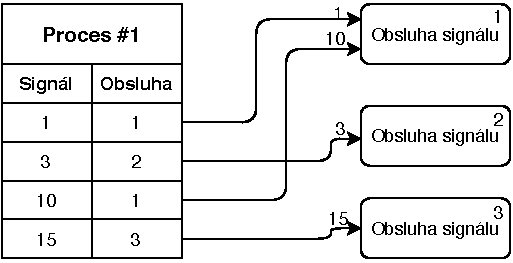
\includegraphics[width=11.5cm]{pdf/register_signal_handler.pdf}}
\caption{Vizualizace tabulky obsluh systémových signálů jednoho procesu}
\label{fig:screen-transition-diagram}
\end{figure}

Při rozeslání signálu jádrem se dle tabulky obsluh každého procesu dohledává, která obsluha se má zavolat. Pokud některý z procesů nemá nastavenou vlastní obsluhu daného signálu, tak se zavolá výchozí obsluha signálu definovaná kernelem.

\subsection{Implementace rour}
Aby bylo možné přesměrovávat výstup jednoho procesu do vstupu jiného, je třeba, aby jádro umožňovalo vytvářet roury, které mají vstup, výstup a paměťový buffer.

Implementace rour představuje rozšíření řešení problému \textit{producent a konzument}. Třída, jejíž instance představují samotné roury, je definována v souborech \texttt{kernel/pipe.h} a \texttt{kernel/pipe.cpp}. V konstruktoru přijímá velikost bufferu, podle které dále inicializuje dva semafory. Volajícímu poskytuje následující metody:

\begin{itemize}

    \item \texttt{std::vector<char> Pipe::Read(size\_t read, bool \&empty)} - tato metoda, která představuje konzumenta a slouží ke čtení požadovaného množství dat z bufferu, přijímá v druhém parametru referenci na booleanskou hodnotu, kterou nastaví na \texttt{true}, pokud byl přečten celý dostupný obsah bufferu a vstup roury byl zavřen. V takový moment již není co číst a nelze očekávat, že do bufferu bude cokoliv zapsáno, protože vstup byl již zavřen.

    \item \texttt{size\_t Pipe::Write(std::vector<char> data)} - tato metoda představující producenta slouží k zapisování předaných dat do bufferu a vrací počet zapsaných bytů. Pokud v průběhu zápisu byl zavřen výstup nebo vstup roury, je zapisování přerušeno.

    \item \texttt{void Pipe::Close\_Out()} - slouží k zavření výstupu, kdy po zavření notifikuje semafory pro zápis i čtení, aby bylo možné oznámit vláknům čekajícím na zápis nebo čtení událost zavření výstupu.

    \item \texttt{void Pipe::Close\_In()} - slouží k zavření vstupu, kdy nejdřív zapíše znak \texttt{EOT} a až poté vstup zavře. 

\end{itemize}

Pro vytvoření rour z uživatelského prostředí slouží systémové volání \texttt{Create\_Pipe}, které vytvoří nový objekt roury, dvakrát jej vloží do tabulky souborů (jedno pro zápis a jednou pro čtení) a vygenerované identifikátory (indexy do souoborové tabulky) zapíše do registrů.


\subsection{Tabulka souborů}
K uložení informací o aktuálně otevřených souborech slouží tzv. tabulka souborů. Taková tabulka v sobě obsahuje seznam všech aktuálně otevřených souborů, kdy každý záznam v tabulce představuje jedno otevření souboru a může obsahovat informaci o způsobu, jakým byl otevřen (např. atributy \texttt{kiv\_os::NFile\_Attribtues}). Tento záznam také obsahuje odkaz na instanci implementace abstraktní třídy \texttt{Generic\_File}, která definuje, jak se z daného souboru čte. V této semestrální práci jsou implementovány následující typy souborů:

\begin{itemize}

    \item soubor souborového systému -- implementován ve třídě \texttt{Filesystem\_File} a v konstruktoru přebírá odkaz na rozhraní souborového systému, kterým může být souborový systém FAT nebo \texttt{procfs}, který slouží ke čtení z tabulky procesů.

    \item soubor vstupu roury -- implementován ve třídě \texttt{Pipe\_In\_File} a v konstruktoru přebírá odkaz na instanci roury. Tento soubor podporuje pouze zápis, a zapisuje do roury.

    \item soubor výstupu roury -- implementován ve třídě \texttt{Pipe\_Out\_File} a v konstruktoru přebírá odkaz na instanci roury. Tento soubor podporuje pouze čtení, a čte z roury.

    \item soubor klávesnice -- implementován ve třídě \texttt{Keyboard\_File} a umožňuje číst z klávesnice, potažmo z konzole. Umožňuje i zápis, který zapisuje do virtuálního bufferu klávesnice.

    \item soubor textového výstupu -- implementován ve třídě \texttt{Tty\_File} a umožňuje zapisovat do konzole.

\end{itemize}

Tato tabulka je implementovaná jako třída obalující \texttt{std::map<kiv\_os::THandle, std::unique\_ptr<Generic\_File>>}. Otevřením nového souboru vznikne v této tabulce nový záznam, a při zavření je z tabulky odebrán.

\begin{table}[ht]
\centering
\begin{tabular}{|l|l|}
\hline
\textbf{Identifikátor} & \textbf{Obecný souborový objekt} \\ \hline
1                      & \texttt{Keyboard\_File}                   \\ \hline
2                      & \texttt{Tty\_File}                        \\ \hline
3                      & \texttt{Pipe\_In\_File}                   \\ \hline
4                      & \texttt{Pipe\_Out\_File}                  \\ \hline
5                      & \texttt{Fs\_File}                         \\ \hline
\end{tabular}
\caption{Ukázka tabulky obecných souborových objektů}
\end{table}

Díky této implementaci je tedy zápis a čtení do souborů jednoduchý, protože logika implementace je volajícímu schovaná -- stačí pouze znát identifikátor požadovaného souboru.

\subsubsection{Operace nad soubory}
Nad soubory lze provádět různé operace pomocí následujících systémových volání:

\begin{itemize}
    \item \texttt{Read\_File} -- vyhledá v tabulce souborů daný soubor a provede čtení,
    \item \texttt{Write\_File} -- vyhledá v tabulce souborů daný soubor a provede zápis,
    \item \texttt{Close\_File} -- vyhledá v tabulce souborů daný soubor, zavře ho a odstraní ho ze souborové tabulky,
    \item \texttt{Seek} -- vyhledá v tabulce souborů daný soubor, a dle zadaných parametrů provede jeho zvětšení nebo změnu aktuální pozice kurzoru,
    \item \texttt{Get\_File\_Attribute} -- vyhledá v tabulce souborů daný soubor, a vrátí jeho atributy,
    \item \texttt{Seek\_File\_Attribute} -- vyhledá v tabulce souborů daný soubor, a změní jeho atributy, 
    \item \texttt{Delete\_File} -- vyhledá dle specifikované cesty v připojených souborvých systémech soubor, a pokud existuje, tak se ho pokusí smazat.
\end{itemize}

\subsection{Obecné rozhraní souborového systému}
Každý souborový systém, který by má být podporován jádrem, musí implementovat rozhraní virtuálního souborového systému. Toto rozhraní je definováno v abstraktní třídě \texttt{VFS}. Definuje hlavičky metod pro následující operace:
\begin{itemize}
    \item vytvoření nové složky
    \item odstranění složky
    \item přečtení obsahu složky
    \item otevření souboru (buď již existujícího nebo nově vytvořeného)
    \item zápis
    \item čtení
    \item odstranění souboru
    \item ověření existence souboru ve specifikované složce 
    \item nastavení a získání atributů souboru 
\end{itemize}

Tato třída implementuje metodu \texttt{generate\_dir\_vector}, která v parametrech přebírá seznam položek složky (seznam struktur \texttt{kiv\_os::TDir\_Entry}) a převede je na seznam znaků (\texttt{char}), aby bylo možné tento seznam přečíst z uživatelského prostoru.

Tento způsob definice rozhraní souborového systému umožňuje flexibilní přidávání dalších podporovaných systémů, kdy stačí pouze naimplementovat dané rozhraní a nadefinovat, na jaké cestě se nachází kořen souborového systému. 

\subsubsection{Ověření existence souboru}
Z uživatelského prostoru může přijít požadavek na otevření souboru, jehož adresa může být specifikována buď jako relativní nebo absolutní. Pro jednodušší práci s adresami se používá typu \texttt{std::filesystem::path} ze standardní knihovny. Pokud byla specifikována relativně, tak se vždy na začátek této adresy ještě přidá aktuální pracovní adresář, a začne ověřování existence jednotlivých komponent cesty.

\noindent Ověření existence cesty \texttt{A} používá následující algoritmus:

\begin{enumerate}
    \item načti komponentu adresy a přidej jí do \texttt{P}
    \item zjisti, jaký souborový systém \texttt{S} se na \texttt{P} používá, 
    \item ověř existenci souboru na cestě \texttt{P} pomocí \texttt{S}
    \item pokud na \texttt{P} neexistuje v \texttt{S} soubor -- \textbf{cesta je neplatná}
    \item pokud existuje a cesta obsahuje další komponentu, běž na \textbf{1.}
    \item pokud existuje a cesta již neobsahuje další komponentu, \texttt{P} \textbf{ukazuje na platný soubor} v \texttt{S}
\end{enumerate}

Při změně aktuálně používaného souborového systému se do ADT struktury zásobník přidá na vrchol dosud používaný souborový systém. V každém souborovém systému se počítá počet zanoření. Zpracování komponenty \texttt{..} snižuje počet zanoření v stromové struktuře složek. Pokud počet zanoření dosáhne nulové hodnoty, tak se ze zásobníku vyjme poslední používaný souborový systém. Využití zásobníku snižuje počet vyhledávání kořenů souborových systémů. 

\subsection{Pracovní adresář} \label{wd}
Pomocí systémových volání \texttt{Set\_Working\_Dir} a \texttt{Get\_Working\_Dir} se mění a získává pracovní adresář aktuálního procesu (tj. toho, který inicializoval systémové volání). Při změně adresáře se pomocí algoritmu ukázaném v podkapitole \ref{wd} kontroluje existence adresáře nacházajícího se na zadané cestě. Dále se také kontroluje, zdali cesta opravdu ukazuje na složku, a ne například na obyčejný soubor.

\subsection{Souborový systém \texttt{procfs}}



- jak se z něj čte
- kde je mountnutý
- sdílená struktura



\section{Závěr}	
% TODO závěr

\end{document}    
